\def\difficulty{3}
\sujet{GANIP}
\index{Frameworks!General Adaptive Neighborhood Image Processing}

\begin{note}This tutorial aims to test the elementary operators of the GANIP framework.

The General Adaptive Neighborhood Image Processing (GANIP) is a mathematical framework for adaptive processing and analysis of gray-tone and color images. An intensity image is represented with a set of local neighborhoods defined for each pixel of the image to be studied. Those so-called General Adaptive Neighborhoods (GANs) are simultaneously adaptive with the spatial structures, the analyzing scales and the physical settings of the image to be addressed and/or the human visual system.
\end{note}


The following figure illustrates the GANs of two points on an image of retinal vessels.

{
	\makeatletter
	\renewcommand\fs@ruled{\def\@fs@cfont{\bfseries}\let\@fs@capt\floatc@ruled
		\def\@fs@pre{\hrule height.8pt depth0pt \kern2pt}%
		\def\@fs@post{\kern2pt\hrule\relax}%
		\def\@fs@mid{\vskip2pt}%
		\let\@fs@iftopcapt\iftrue}
	\makeatother
\begin{figure}[htbp]
\centering
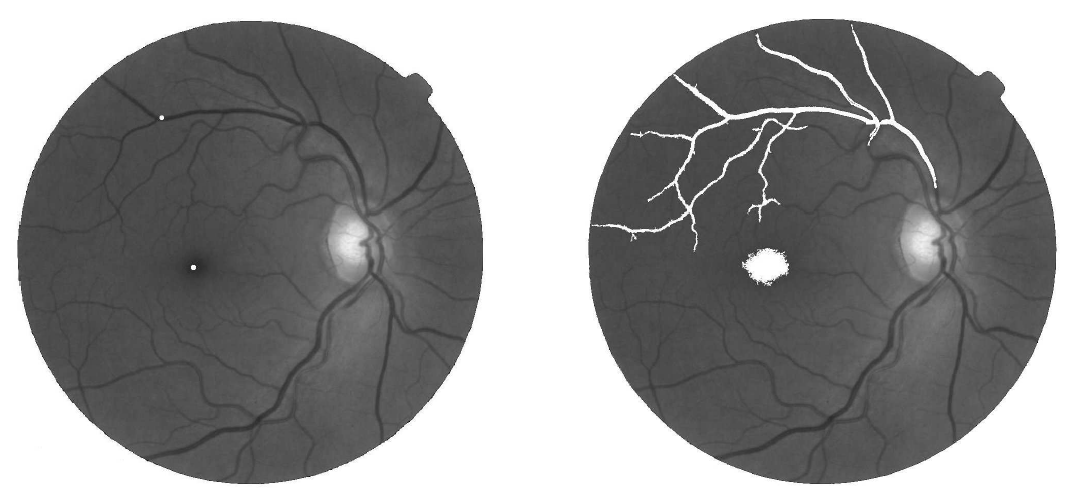
\includegraphics[width=.7\linewidth]{retinaGAN.png}
\end{figure}
}

The GANs are then used as adaptive operational windows for local image transformations (morphological filters, rank/order filters...) and for local image analysis (local descriptors, distance maps...).


\noindent The different processes will be applied on the following gray-tone images:
\begin{figure}[htbp]
\centering\caption{Two example images for testing the GAN framework.}
\subfloat[lena]{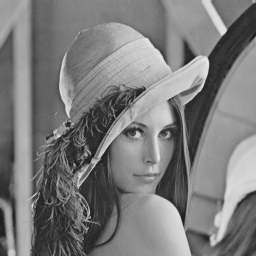
\includegraphics[width=.45\linewidth]{lena256.png}}
\hfill
\subfloat[cement paste (2-D section / X-ray tomography)]{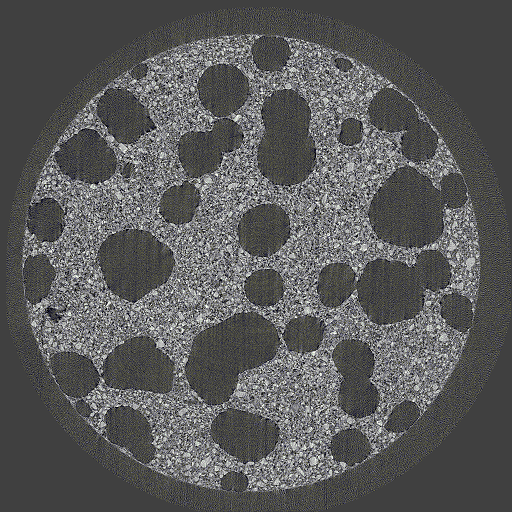
\includegraphics[width=.45\linewidth]{ciment.png}}
\label{fig:ganip:examples}
\end{figure}


\section{GAN}
Let $f$ be a gray-tone image. The GAN of a point $x$ using the luminance criterion and the homogeneity tolerance $m$ within the CLIP framework is defined as:
\begin{eqnarray}
V_m^f(x)=C_{\{y; |f(y)-f(x)|\leq m\}}(x)
\end{eqnarray}
where $C_X(x)$ denotes the connected component of $X$ holding $x$.
\begin{qbox}
\begin{enumerate}
	\item Load the image 'lena' and compute the GAN of a selected point in the image.
	\item Look at the influence of the homogeneity tolerance.
	\item Compute the GAN of different points and comment.
\end{enumerate}
\end{qbox}


\section{GAN Choquet filtering}\index{Filtering!Choquet}
The Choquet filters generalize the rank-order filters.
In this exercise, we are going to implement some GAN Choquet filters such as the GAN mean operator. For each point $x$ of the image, the mean value of all the intensities of the points inside the GAN of $x$ is computed. So, a first algorithm consists in making a loop on the image points for computing the different GAN and the mean intensity values, but it is time consuming. Nevertheless, by using some properties of the GAN (particularly the one giving that iso-valued points can have exactly the same GAN), it is possible to create a second algorithm by making a loop on the gray-tone range:

{\SetCustomAlgoRuledWidth{0pt}
\begin{algorithm}[htbp]
\SetAlgoLined
\SetKw{Set}{set}
\KwData{original (8-bit) image $f$, homogeneity tolerance $m$}
\KwResult{GAN mean filtered image $g$}
\For{$s=0$ \KwTo $255$}{
$seed=$ points $x$ with intensity $f(x)=s$;\\
$thresh=$ points $y$ with intensity satisfying $s-m\leq f(y) \leq s+m$;\\
$threshGAN=$ connected components of $thresh$ holding $seed$;\\
\ForEach{label of $threshGAN$}{
$currentLabel=$ current connected component of $threshGAN$;\\
$meanValue=$ intensity mean value of the image points inside $currentLabel$;\\
\Set $g(x)=meanValue$ to the points $x$ of $seed$ belonging to $currentLabel$;\\
}
}
\end{algorithm}
}

\begin{qbox}
\begin{enumerate}
	\item Implement the proposed algorithm.
	\item Test this operator on the 'lena' image with different homogeneity tolerances.
	\item Compare the result with a classical mean filtering.
\end{enumerate}
\end{qbox}

\begin{mcomment}
\begin{mremark}
 See \minline{imfilter}.
\end{mremark}
\end{mcomment}

\begin{pcomment}
\begin{premark}
 See \pinline{scipy.ndimage.filters}.
\end{premark}
\end{pcomment}



\section{GAN morphological filtering}
\index{Mathematical Morphology!General Adaptive Neighborhood}
As previously explained, it is also possible to compute the GAN dilation and GAN erosion by making a loop on the gray-tone range. The algorithm for the GAN dilation is:

\begin{algorithm}[H]
\SetAlgoLined
\SetKw{Set}{set}
\KwData{original (8-bit) image $f$, homogeneity tolerance $m$}
\KwResult{GAN dilated image $g$}
\Set $g(x)=0$ for all points $x$;\\
\For{$s=0$ \KwTo $255$}{
$seed=$ points $x$ with intensity $f(x)=s$;\\
$thresh=$ points $y$ with intensity satisfying $s-m\leq f(y) \leq s+m$;\\
$threshGAN=$ connected components of $thresh$ holding $seed$;\\
\ForEach{label of $threshGAN$}{
$currentLabel=$ current connected component of $threshGAN$;\\
$maxValue=$ intensity maximum value of the image points inside $currentLabel$;\\
\Set $g(x)=max(g(x),maxValue)$ to the points $x$ belonging to $currentLabel$;\\
}
}
\caption{GAN dilation}
\end{algorithm}
The algorithm for the GAN erosion is similar.
\begin{qbox}
\begin{enumerate}
	\item Implement the GAN dilation and GAN erosion.
	\item Test this operator on the 'lena' image with different homogeneity tolerances.
	\item Compare the results with the classical morphological dilation and erosion..
	\item Compute, test, compare and check the properties (idempotence, ex\-ten\-si\-vi\-ty/anti-extensivity) of the GAN opening and GAN closing.
\end{enumerate}
\end{qbox}

\begin{mcomment}
 \begin{mremark}
  Compare with the functions \minline{imdilate} and \minline{imerode}.
 \end{mremark}
\end{mcomment}

\begin{pcomment}
 \begin{premark}
  Compare with the functions \pinline{dilation} and \pinline{erosion} from \pinline{skimage.morphology}.
 \end{premark}
\end{pcomment}
